\documentclass[12pt]{article}
\usepackage[utf8]{inputenc}
\usepackage[letterpaper, margin=1in]{geometry}
\usepackage{graphicx}
\usepackage{mathptmx}
\usepackage{float}
\usepackage[cmex10]{amsmath}
\usepackage{amsthm,amssymb}
\usepackage{url}
\urlstyle{same} 
\def\UrlBreaks{\do\/\do-}
\usepackage{breakurl}
\usepackage{fancybox}
\usepackage{breqn}
\usepackage{array}
\usepackage{caption}
\usepackage{subcaption}
\usepackage{comment}
\usepackage[english]{babel}
\usepackage[acronym,nomain]{glossaries} % list of acronyms
\usepackage{xurl}
\usepackage{cite} % math and engineering style citations
\usepackage{multicol}
\usepackage{multirow}
\usepackage{mathptmx}
\usepackage{float}
\usepackage{lipsum}
\usepackage{framed}
\usepackage[T1]{fontenc}
\usepackage[pdfpagelabels,pdfusetitle,colorlinks=false,pdfborder={0 0 0}]{hyperref}
\usepackage{algorithm}
\usepackage{algpseudocode}

% draw a frame around given text
\newcommand{\framedtext}[1]{%
	\par%
	\noindent\fbox{%
		\parbox{\dimexpr\linewidth-2\fboxsep-2\fboxrule}{#1}%
	}%
}

\renewcommand{\arraystretch}{1.2}

\sloppy

\newcolumntype{C}[1]{>{\centering\let\newline\\\arraybackslash\hspace{0pt}}m{#1-2\tabcolsep}}

\title{Routing-Based Methodology for Evaluation of \gls{evse} Networks}
\author{Aaron I. Rabinowitz}
\date{}

\newacronym{ghg}{GHG}{Green-House Gas}
\newacronym{fe}{FE}{Fuel Economy}
\newacronym{ee}{EE}{Energy Economy}
\newacronym{epa}{EPA}{Environmental Protection Agency}
\newacronym{oem}{OEM}{Original Equipment Manufacturer}
\newacronym{ice}{ICE}{Internal Combustion Engine}
\newacronym{icv}{ICV}{Internal Combustion Vehicle}
\newacronym{icev}{ICEV}{Internal Combustion Engine Vehicle}
\newacronym{em}{EM}{Electric Motor}
\newacronym{hev}{HEV}{Hybrid Electric Vehicle}
\newacronym{ev}{EV}{Electric Vehicle}
\newacronym{phev}{PHEV}{Plug-in Hybrid Electric Vehicle}
\newacronym{lrphev}{LR-PHEV}{Long Range PHEV}
\newacronym{srphev}{SR-PHEV}{Short Range PHEV}
\newacronym{mhev}{MHEV}{Mild Hybrid Electric Vehicle}
\newacronym{pev}{PEV}{Plug-in Electric Vehicle}
\newacronym{bev}{BEV}{Battery Electric Vehicle}
\newacronym{cbev}{CBEV}{City BEV}
\newacronym{afv}{AFV}{Alternative Fuel Vehicle}
\newacronym{fcev}{FCEV}{Fuel Cell Electric Vehicle}
\newacronym{cav}{CAV}{Connected Autonomous Vehicle}
\newacronym{fc}{FC}{Fuel Consumption}
\newacronym{ec}{EC}{Energy Consumption}
\newacronym{dtto}{DTTO}{Discrete Time Trajectory Optimization}
\newacronym{udto}{UDTO}{Uniformly Discretized Trajectory Optimization}
\newacronym{sto}{STO}{Spline Trajectory Optimization}
\newacronym{rbed}{RBED}{Rules-Based Eco-Driving}
\newacronym{cidm}{CIDM}{Cooperative Intelligent Driver Model}
\newacronym{idm}{IDM}{Intelligent Driver Model}
\newacronym{soc}{SOC}{State of Charge}
\newacronym{ocp}{OCP}{Optimal Control Problem}
\newacronym{ttc}{TTC}{Time-To-Collision}
\newacronym{dp}{DP}{Dynamic Programming}
\newacronym{ga}{GA}{Genetic Algorithm}
\newacronym{sdm}{SDM}{Smart Driver Model}
\newacronym{v2i}{V2I}{Vehicle to Infrastructure}
\newacronym{v2v}{V2V}{Vehicle to Vehicle}
\newacronym{v2x}{V2X}{Vehicle to Everything}
\newacronym{hil}{HIL}{Hardware In Loop}
\newacronym{pso}{PSO}{Particle Swarm Optimization}
\newacronym{dt}{DT}{Direct Transcription}
\newacronym{oedt}{OEDT}{Optimal Eco-Driving Trace}
\newacronym{fods}{FODS}{Forward Object Detection System}
\newacronym{cas}{CAS}{Collision Aviodance System}
\newacronym{acc}{ACC}{Adaptive Cruise Control}
\newacronym{obu}{OBU}{On-Board Unit}
\newacronym{rsu}{RSU}{Road-Side Unit}
\newacronym{sae}{SAE}{Society of Automotive Engineers}
\newacronym{adas}{ADAS}{Advanced Driver Assistance System}
\newacronym{edc}{EDC}{Eco-Driving Control}
\newacronym{lv}{LV}{Lead Vehicle}
\newacronym{ss}{SS}{Segment Speeds}
\newacronym{hs}{HS}{Historical Speeds}
\newacronym{spat}{SPAT}{Signal Phase and Timing}
\newacronym{map}{MAP}{Positions of Subsequent Traffic Lights}
\newacronym{al2n}{AL2N}{Acceleration L\textsuperscript{2} Norm}
\newacronym{rpc}{RPC}{Road Power Cost}
\newacronym{bpc}{BPC}{Battery Power Cost}
\newacronym{fecc}{FECC}{Fitted Equivalent Consumption Cost}
\newacronym{ipopt}{IPOPT}{Interior-Point Optimization}
\newacronym{dtnlp}{DTNLP}{Discreet-Time Non-Linear Programming}
\newacronym{snlp}{SNLP}{Spline Non-Linear Programming}
\newacronym{sga}{SGA}{Spline Genetic Algorithm}
\newacronym{spso}{SPSO}{Spline Particle Swarm Optimization}
\newacronym{2sdp}{2SDP}{2 State Dynamic Programming}
\newacronym{aos}{AOS}{Approximate Optimal Spline}
\newacronym{pchip}{PCHIP}{Piecewise Cubic Hermitic Interpolation Polynomial}
\newacronym{nrel}{NREL}{National Renewable Energy Laboratory}
\newacronym{fastsim}{FASTSim}{Future Automotive Systems Technology Simulator}
\newacronym{mfei}{MFEI}{Mean Fuel Economy Improvement}
\newacronym{pas}{PAS}{Percent Acceptable Solutions}
\newacronym{mrt}{MRT}{Mean Run-Time}
\newacronym{mpc}{MPC}{Model Predictive Control}
\newacronym{adp}{ADP}{Approximate Dynamic Programming}
\newacronym{rl}{RL}{Reinforcement Learning}
\newacronym{mbrl}{MBRL}{Model Based Reinforcement Learning}
\newacronym{nlp}{NLP}{Non-Linear Programming}
\newacronym{nhtsa}{NHTSA}{National Highway Traffic Safety Administration}
\newacronym{aeb}{AEB}{Automatic Emergency Braking}
\newacronym{tsdc}{TSDC}{Transportation Secure Data Center}
\newacronym{anl}{ANL}{Argonne National Lab}
\newacronym{d3}{D\textsuperscript{3}}{Downloadable Dynamometer Database}
\newacronym{cd}{C\textsubscript{D}}{Coefficient of Drag}
\newacronym{crr}{C\textsubscript{RR}}{Coefficient of Rolling Resistance}
\newacronym{mape}{MAPE}{Mean Absolute Percentage Error}
\newacronym{evse}{EVSE}{Electric Vehicle Supply Equipment}
\newacronym{ld}{LD}{Light Duty}
\newacronym{md}{MD}{Medium Duty}
\newacronym{hd}{HD}{Heavy Duty}
\newacronym{mdhd}{MD/HD}{Medium Duty / Heavy Duty}
\newacronym{inrix}{INRIX}{}
\newacronym{epri}{EPRI}{Electric Power Research Institute}
\newacronym{nhts}{NHTS}{National Highway Transportation Survey}
\newacronym{usa}{USA}{United States of America}
\newacronym{sof}{SOF}{State of Fuel}
\newacronym{hc}{HC}{Home Charging}
\newacronym{bc}{BC}{Battery Capacity}
\newacronym{dcl}{DCL}{Destination Charger Likelihood}
\newacronym{ercr}{ERCR}{En-Route Charging Rate}
\newacronym{ercp}{ERCP}{En-Route Charging Penalty}
\newacronym{ftc}{FTC}{Fuel Tank Capacity}
\newacronym{ftp}{FTP}{Fuling Time Penalty}
\newacronym{psrc}{PSRC}{Puget Sound Regional Council}
\newacronym{bts}{BTS}{Bureau of Transportation Statistics}
\newacronym{happ}{HAPP}{Household Activity Pattern Problem}
\newacronym{chts}{CHTS}{California Houslehold Travel Survey}
\newacronym{dcfc}{DCFC}{DC Fast Charging}
\newacronym{liion}{Li-Ion}{Lithium-Ion}
\newacronym{lvl2}{LVL 2}{DC Level 2}
\newacronym{oems}{OEMS}{Optimal Energy Management Strategies}
\newacronym{poems}{POEMS}{Predictive Optimal Energy Management Strategies}
\newacronym{vpoems}{VP-OEMS}{Velocity Prediction enabled Optimal Energy Management Strategies}
\newacronym{gnss}{GNSS}{Global Navigational Satellite System}
\newacronym{obd2}{OBD-II}{On-Board Diagnostics II}
\newacronym{csu}{CSU}{Colorado State University}
\newacronym{wes}{WES}{Weight Efficiency Score}
\newacronym{gvwr}{GVWR}{Gross Vehicle Weight Rating}
\newacronym{fha}{FHA}{Federal Highway Administration}
\newacronym{vius}{VIUS}{Vehicle Inventory and Use Survey}
\newacronym{eod}{EOD}{End of Day}
\newacronym{osrm}{OSRM}{Open-Source Routing Machine}
\newacronym{vrp}{VRP}{Vehicle Routing Problem}
\newacronym{evrp}{EVRP}{Electric Vehicle Routing Problem}
\newacronym{tsp}{TSP}{Traveling Salesman Problem}
\newacronym{can}{CAN}{Controller Area Network}
\newacronym{lstm}{LSTM}{Long Short-Term Memory}
\newacronym{ann}{ANN}{Artificial Neural Network}
\newacronym{ml}{ML}{Machine Learning}
\newacronym{fcdp}{FC-DP}{Full Cycle Dynamic Programming}
\newacronym{ppmpc}{PP-MPC}{Perfect Prediction Model Predictive Control}
\newacronym{rpmpc}{RP-MPC}{Real Prediction Model Predictive Control}
\newacronym{cvmpc}{CV-MPC}{Constant Velocity Model Predictive Control}
\newacronym{mae}{MAE}{Mean Absolute Error}
\newacronym{fsmvrp}{FSMVRP}{Fleet Size and Mix Vehicle Routing Problem}
\newacronym{mcvrp}{MCVRP}{Monte-Carlo Vehicle Routing Problem}
\newacronym{ppf}{PPF}{Percent Point Function}
\newacronym{ccdng}{CCDNG}{Completely Connected Directional Network Graph}
\newacronym{sho}{SHO}{Spline Heuristic-Optimal}
\newacronym{npv}{NPV}{Net Present Value}
\newacronym{tco}{TCO}{Total Cost of Ownership}
\newacronym{mtk}{MTK}{Metric-Ton-Kilometer}
\newacronym{lco}{LCO}{Levelized Cost of Ownership}
\newacronym{lcod}{LCOD}{Levelized Cost of Driving}
\newacronym{sme}{SME}{Subject Matter Expert}
\newacronym{doe}{DOE}{Deparment of Energy}
\newacronym{vmt}{VMT}{Vehicle Miles Traveled}
\newacronym{dot}{DOT}{Department of Transportation}
\newacronym{ltl}{LTL}{Less Than Truckload}
\newacronym{lpcp}{LPCP}{Lost Payload Capacity Portion}
\newacronym{chaas}{ChaaS}{Charging as a Service}
\newacronym{tou}{TOU}{Time of Use}
\newacronym{ocs}{OCS}{Optimal Charging Strategy}
\newacronym{soe}{SOE}{State of Energy}
\newacronym{ltp}{LTP}{Lost Time Portion}
\newacronym{yd}{YD}{Yearly Distance}
\newacronym{dd}{DD}{Daily Distance}
\newacronym{vnr}{VNR}{Vehicle Nominal Range}
\newacronym{nyo}{NYO}{Number of Years of Ownership}
\newacronym{ap}{AP}{Age at Purchase}
\newacronym{dpm}{DPM}{Diesel Price Multiplier}
\newacronym{epm}{EPM}{Electricity Price Multiplier}
\newacronym{evsep}{EVSEP}{EVSE Premium}
\newacronym{pe}{PE}{Payload Exemption}
\newacronym{bpp}{BPP}{Battery Pack Pricing}
\newacronym{my}{MY}{Model Year}
\newacronym{ipfn}{IPFN}{Iterative Proportional Fitting with N dimensions}
\newacronym{dco}{DCO}{Discretized Control Optimization}
\newacronym{pto}{PTO}{Polynomial Trajectory Optimization}
\newacronym{slsqp}{SLSQP}{Sequential Least Squares Programming}
\newacronym{aer}{AER}{All Electric Range}
\newacronym{msrp}{MSRP}{Manufacturer Recommended Sales Price}
\newacronym{afdc}{AFDC}{Alternative Fuels Data Center}
\newacronym{uf}{UF}{Utility Factor}
\newacronym{hov}{HOV}{Hich Occupancy Vehicle}
\newacronym{lp}{LP}{Linear Problem}
\newacronym{qp}{QP}{Quadratic Problem}
\newacronym{sp}{SP}{Stochastic Problem}
\newacronym{slp}{S-LP}{Stochastic Linear Problem}
\newacronym{milp}{MILP}{Mixed Integer Linear Problem}
\newacronym{smilp}{S-MILP}{Stochastic Mixed Integer Linear Problem}
\newacronym{los}{LOS}{Level of Service}
\newacronym{v2s}{V2S}{Vehicle-to-Structure}
\newacronym{v2g}{V2G}{Vehicle-to-Grid}
\newacronym{gacm}{GACM}{Grid-Aware Charge Management}
\newacronym{iso}{ISO}{Independent System Operator}
\newacronym{dcopf}{DC-OPF}{DC Optimal Power Flow}
\newacronym{lmp}{LMP}{Location Marginal Price}
\newacronym{gcc}{GCC}{Giant Connected Component}
\newacronym{hjb}{HJB}{Hamilton-Jacobi-Bellman}
\newacronym{pdf}{PDF}{Probability Distribution Function}
\newacronym{scram}{SCRAM}{Stochastic Cost with Risk Allowance Minimization}
\newacronym{scramd}{SCRAM-D}{SCRAM-Dijkstra}
\newacronym{scramb}{SCRAM-B}{SCRAM-Bellman}
\newacronym{rsic}{RSIC}{Range-Sensitive Information Centrality}
\newacronym{rsbc}{RSBC}{Range-Sensitive Betweenness Centrality}
\newacronym{ras}{RAS}{Range Addition Station}

\makeglossaries

\begin{document}

\maketitle

\section*{Introduction}

When discussing transportation networks, one must consider several linked and mutually supporting networks including road, rail, marine, and air infrastructure in addition to those energy and information networks which allow for vehicles to function. Multiple support systems are required for the efficient and economical operation of vehicles which underpins modern economies and standards of living. The various networks are coincident at a subset of nodes but, otherwise, may be operated in various manners by dissimilar stakeholders in service of divergent objectives. none of the related networks is a subset of any other but all share dependence relationships which may be asymmetrical.

The mode of vehicles in today's transportation sector, whether passenger or cargo oriented, are \glspl{icev} but a growing number of these vehicles are being supplanted by \glspl{pev}. This shift necessitates a re-alignment of the networks underpinning travel as the nodes of interaction between physical infrastructure and the energy system are incompatible between \glspl{icev} and \glspl{bev}. \glspl{icev} receive energy from a fuel distribution network which connects extraction operations to processing plants and ultimately to distribution stations. The fueling network is inherently inefficient due to constraints on the location of extraction sites, the economies of scale and access related to processing sites, and the requirement to expend fuel to transport fuel to end user locations which are widely distributed. It is, nevertheless, the case that this network has been subject to tremendous amounts of capital expenditure and operational optimization such that it's function and economic viability is ensured as long as extricable fuel supplies continue to be discovered and fuel-burning vehicles continue to be used.

\glspl{pev}, by contrast, draw energy from the electricity distribution network which also powers static loads such as those from buildings. Also the recipient of substantial and continuous investment, the power grid has been, historically, optimized to meet demand from buildings via the utilization of dispatchable resources including fuel-burning power plants. As the number of \glspl{pev} continues to rise, the load required to power these vehicles will become a greater portion of the overall load required. The interaction between vehicles and the power grid is heavily bound by constraints at coincident nodes and within their valency. Limitations exist on power transfer rates between the charger and battery as well as between the charger and power generation as a function of the distribution grid.

The most salient difference between the \gls{icev} fuel delivery network and the \gls{evse} network is at the interaction points. There are many more fueling stations in any given region of a developed country than public chargers. On the other hand, there are many more private charging locations than private fueling locations. \glspl{pev} are able to charge at low rates from many nodes including homes and buildings which are connected to the grid. Low rate charging is preferable for several reasons including lower costs per kWh and lower battery degradation. High rate charging is generally reserved for situations wherein charge time is relevant such as on itineraries whose distance is in excess of a vehicle's single charge range or for daily use by people unable to charge at home/work. The multifaceted nature of \gls{pev} charging contrasts to that of \gls{icev} fueling which takes lace at public access stations and at similar rates for the vast majority of fueling events. A significant portion of \gls{pev} users can accomplish most charging without relying on public-access stations and these are encourages to maintain this behavior. The multi-tiered "charging pyramid" dictates that fewer public-access fast charging stations can be supported for a given number of \glspl{pev} compared to fueling stations and \glspl{icev}.

As a result of the economic realities of charging stations, increases in network cardinality have, generally, been driven by incentives. The goal of these incentives is to create a network of public-access charging stations which is sufficiently ubiquitous and reliable that potential buyers will view \glspl{pev} as completely viable vehicles. A secondary goal would be to incentivise an efficient distribution of these stations such that profitable operations can be maintained after the subsidy period runs out. This document outlines methods of analysis for these networks which are fundamental and extensible and provide insights which can be used for further roll-out.

\section*{\gls{evse} Network}

For \gls{evse} networks, the nodes are charging stations. The focus of this document is long distance travel and , thus, only \gls{dcfc} nodes will be considered. Because interoperability between vehicles and chargers is not universal, the network will look different for different types of vehicle. An \gls{evse} network's links are ephemeral end vehicle-dependent. Links exist between all chargers and all other chargers within range. This creates a highly connected network with significant locality. A key feature of any \gls{evse} network is the low probability of availability at all nodes. Chargers are unreliable and may be unavailable for reasons including hardware and software faults, physical blockage, plug damage, payment system failures, and occupation. Because \gls{pev} fast charging events take a relatively long amount of time compared to \gls{icev} fueling events and the relatively low number of plugs per station and stations per mile of road network, the probability of plug occupation is high, especially for central nodes. This can lead to a frustrating driving experience as limited prior knowledge of charger availability is the norm.

Constructing an \gls{evse} network requires the locations of usable chargers, vehicle usable range, and a road network which has nodes coincident with the chargers, or nearly so. In this document, the road network will be referred to as the atlas. The links of the \gls{evse} network are constructed by finding the lowest cost (however defined) route for all node pairs which do not violate cost limits. Routing along the network involves the additional step of adding origins and destinations to the network in the same manner as adding chargers.

\subsection*{Generic Example}

Shown in Figure \ref{fig:random_graph} is a randomly generated graph ($G = \{V, E\}$) with a cardinality of $N = 100$ on a 100 km by 100 km area with a link probability determined by $P(E|L_E) = e^{-L / S}$ where $E$ is the link from $V_i$ to $V_j$, $L_E$ is the Pythagorean distance between $V_i$ and $V_j$, and $S$ is a characteristic distance, (10 km in this case). Among the nodes in the graph, one has been designated the origin, five have been assigned as destinations, and ten have been assigned as chargers.

\begin{figure}[H]
	\centering
	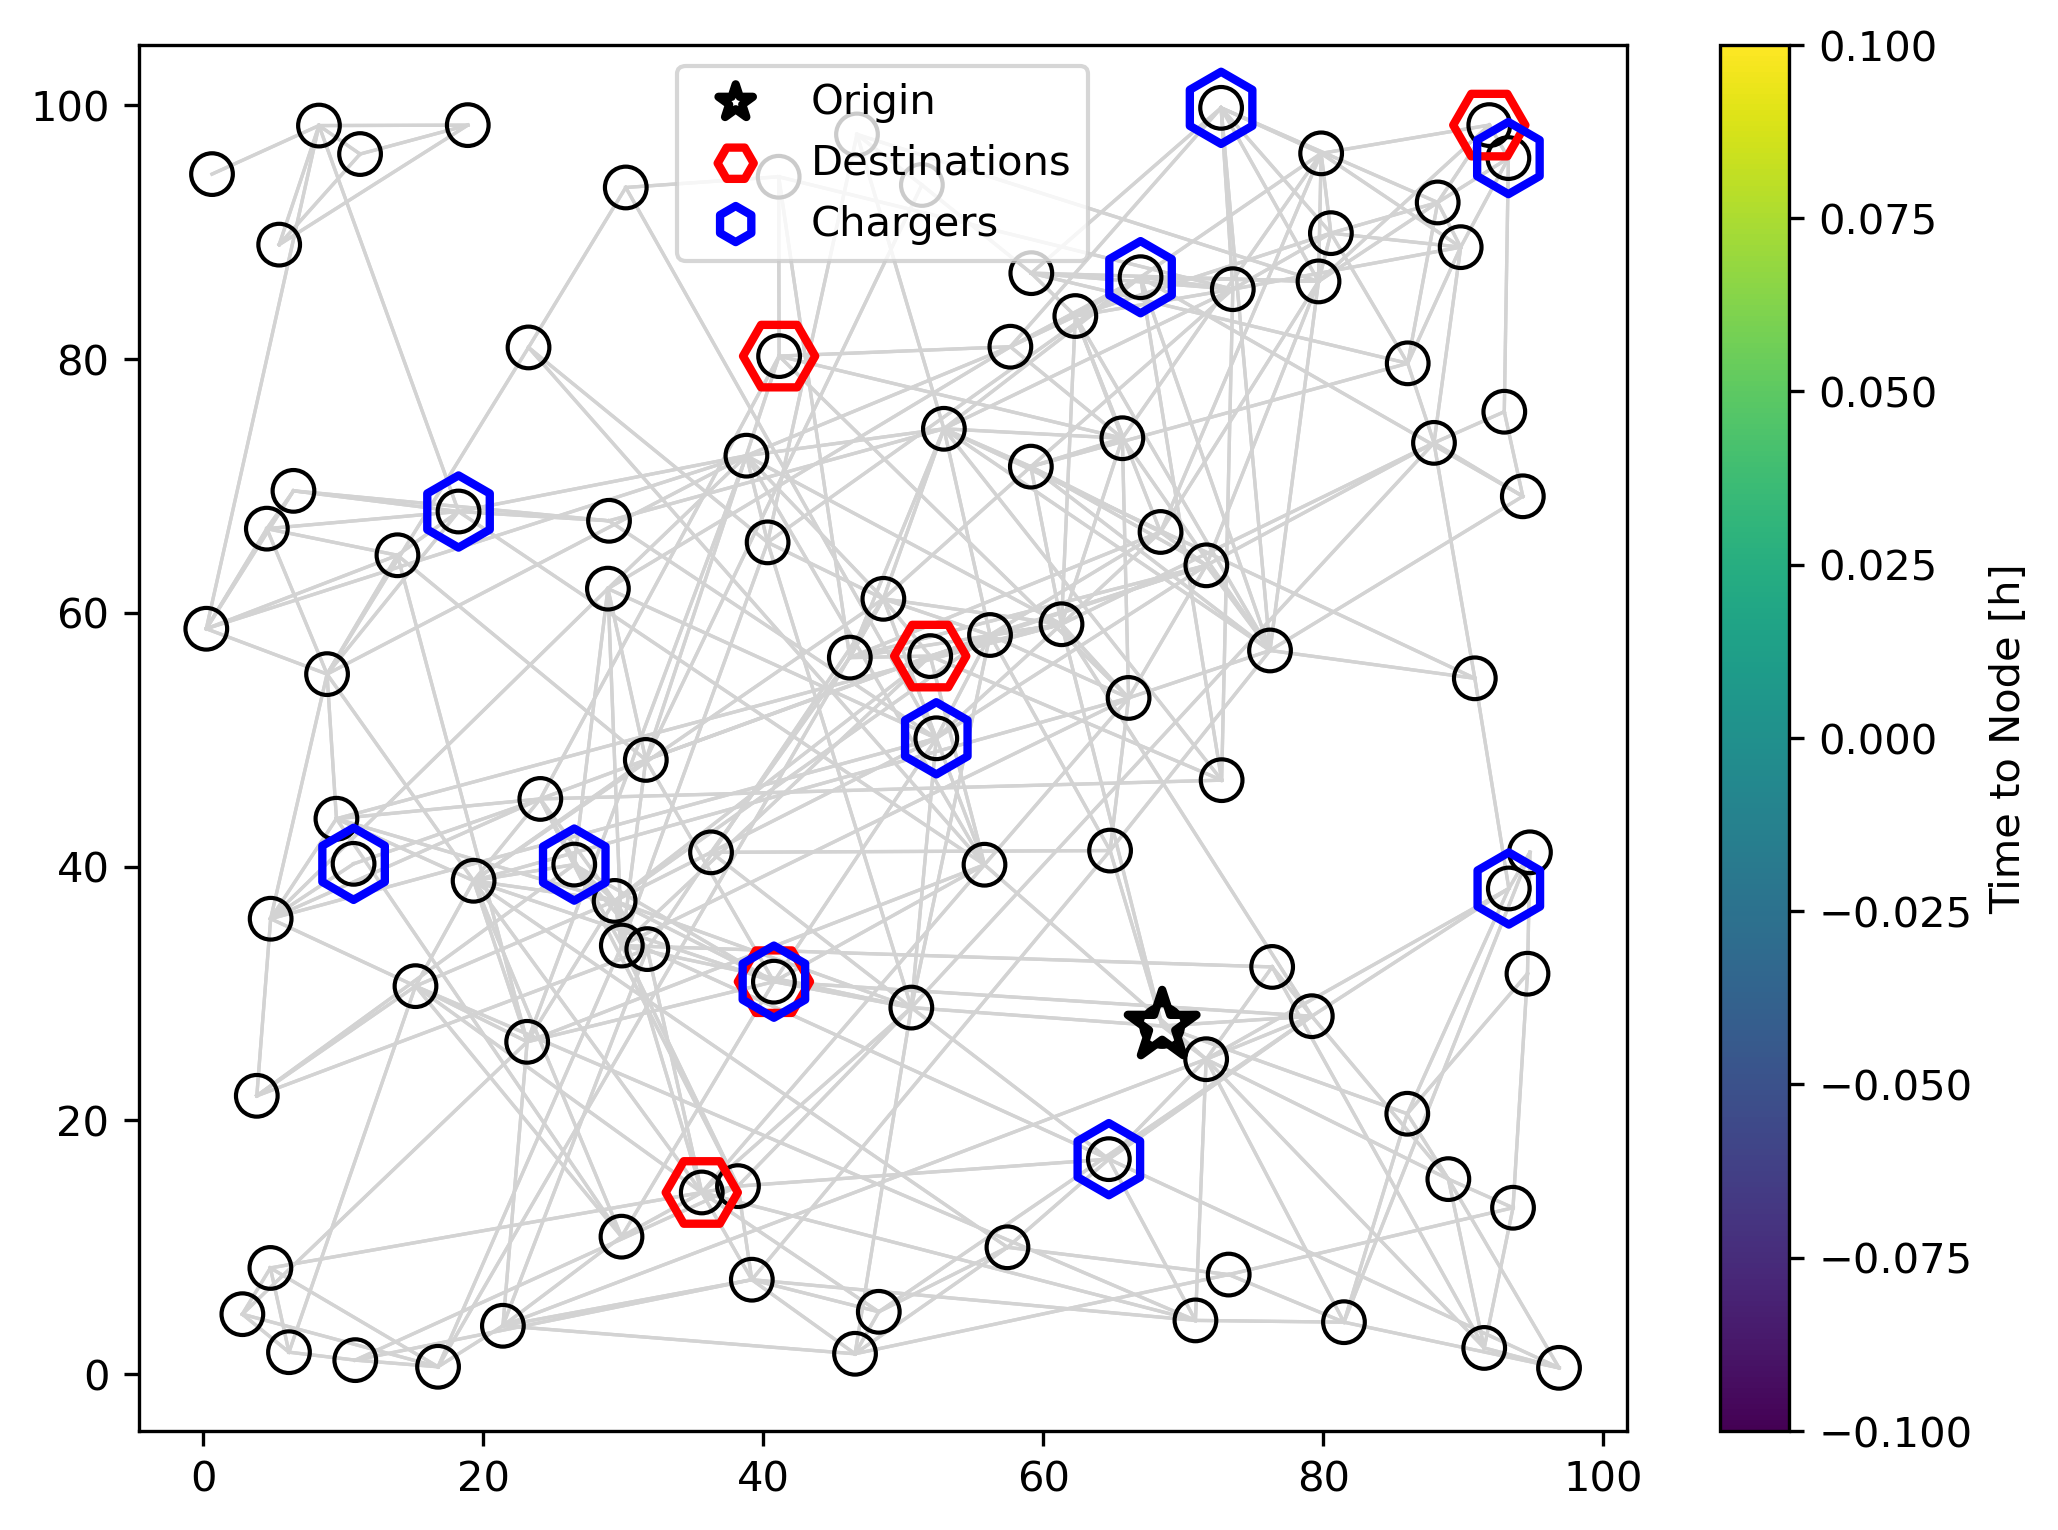
\includegraphics[width = \linewidth * 2 / 3]{figs/random_graph.png}
	\caption{Randomly generated graph with cardinality of 100 with 1 origin, 5 destinations, and 10 chargers.}
	\label{fig:random_graph}
\end{figure}

The links are traversed at speeds randomly selected from $\{35, 55, 90, 105\}$ kph. Like a real road network, all nodes are connected to the \gls{gcc} but not directly to all others. Because the random graph is based on nodes drawn from a uniform random distribution, the distances between nodes should be normally distributed. Because the probability of a given link is a function of distance, one would also expect the nodes in the middle to have the highest valency and for valency to be Poisson distributed and this is, indeed, the case.

\subsection*{California Example}

The state of California contains 1,618 towns and cities, collectively referred to as places, per the US Census Bureau and 1,906 public DC charging stations per \gls{afdc}. Itineraries entirely contained in California will originate and terminate at California places. If additional range is needed beyond the remaining range at the start of the trip, \glspl{ev} will utilize one of the DC charging stations. The places and stations are completely connected by roads. Thus, an entity atlas can be computed by routing from each entity to each entity. For the purposes of reducing computation time and memory requirements, a limit on link ranges can be implemented which may result in a non-completely-connected entity atlas which should, nevertheless, be entirely contained within the \gls{gcc}. The components of the California entity atlas are shown in Figure \ref{fig:california_entity_atlas}.

\begin{figure}[H]
	\centering
	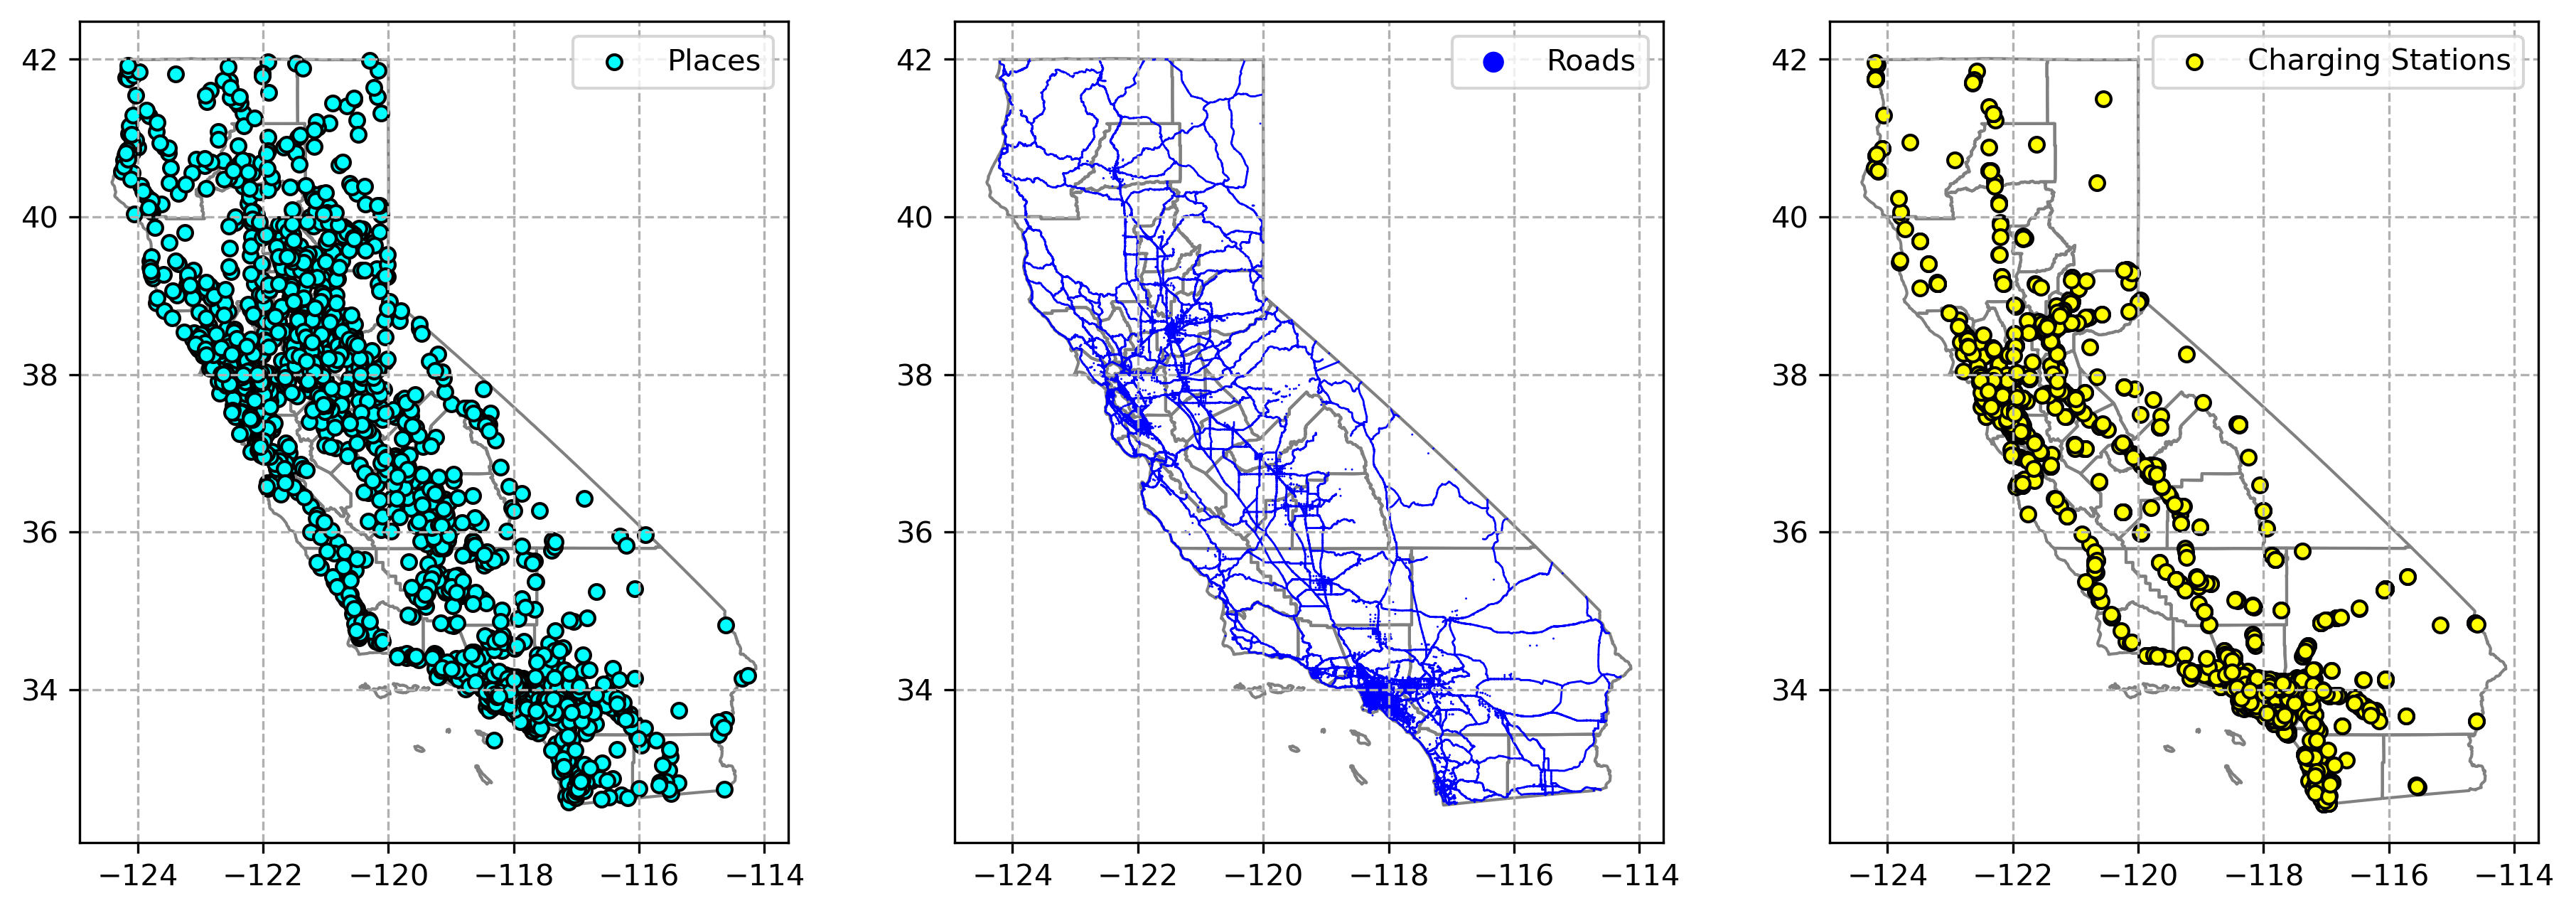
\includegraphics[width = \linewidth]{figs/California_Places_Chargers.png}
	\caption{Components of California entity atlas}
	\label{fig:california_entity_atlas}
\end{figure}

\section*{Routing}

\subsection*{Background}

For a graph $G=\{V,E\}$ where $O\in V$ is an origin and $D\in V$ is a destination, there is an optimal route $R^* = \{O, \Phi_0, \dots, \Phi_N, D\}| R^*\subset V$ such that $J^*=F(G,R^*)$ is the global minimum value of $J$ for routing cost function $J = F(G,R)$. There are, in essence, two approaches to finding $R^*$, Dijkstra's method and Bellman's method. Both methods are founded on the \gls{hjb} equation

\begin{equation}
	J_k = F(U_k,\dots) + F(U^*_{k+1},\dots)
\end{equation}

which states that the cost of a given control at the current step is the sum of the cost of the control and the cost of the optimal control at the next step subject to the control for a time-varying \gls{ocp}. A corollary is that the optimal control at a given step is influenced by the optimal controls at all following steps. Dijkstra's method implements this concept via forward induction where Bellman's method implements this concept via backward induction followed by forward evaluation. The methods are diagrammed in Figure \ref{fig:dijkstra_bellman} and algorithms for both can be found in the Appendix.

\begin{figure}[H]
	\centering
	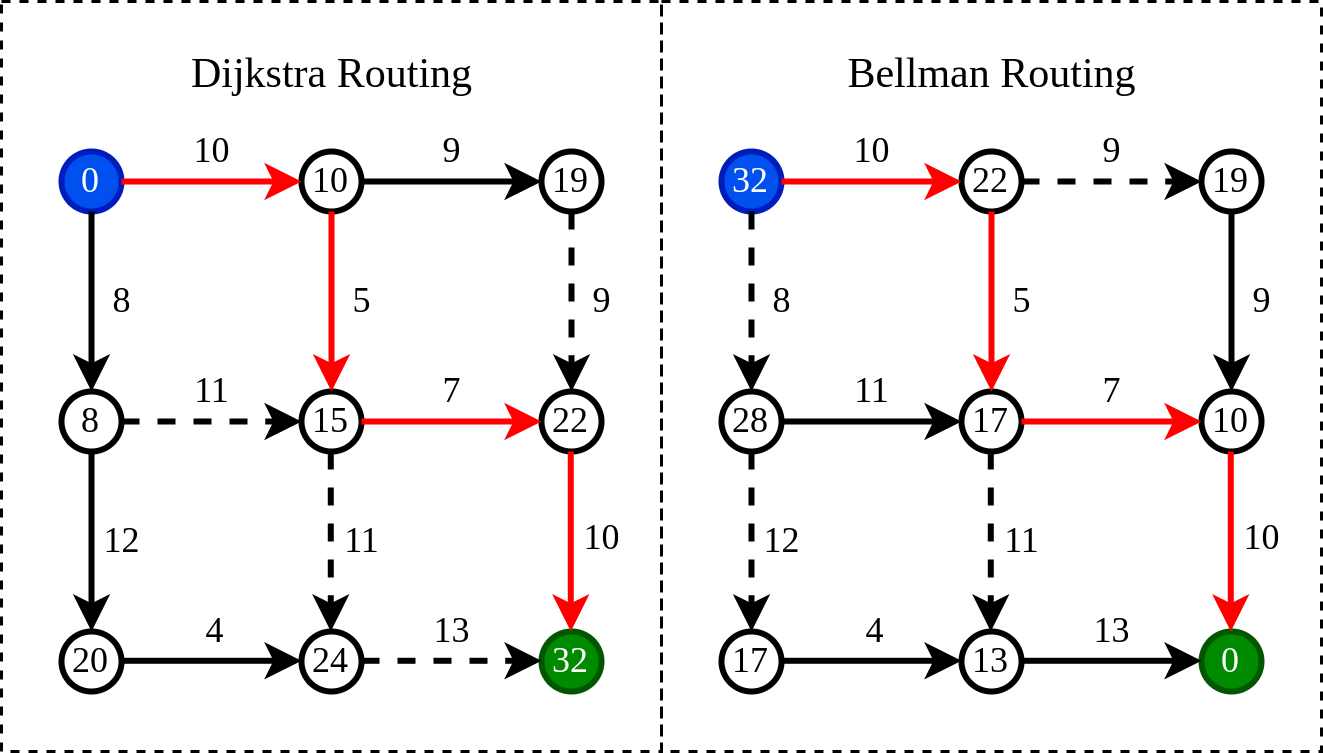
\includegraphics[width = \linewidth]{figs/routing_diagram.png}
	\caption{Comparison between Dijkstra and Bellman routing methods}
	\label{fig:dijkstra_bellman}
\end{figure}

It is worth noting that \textbf{Dijkstra's algorithm creates a tree from a single origin to all destinations} where \textbf{Bellman's algorithm creates a tree from all origins to a single destination}. The optimal paths created by both algorithms for a single O/D pair on a common graph will usually be the same unless there are many similarly expensive paths. The path produced by Bellman's method will be the globally optimal path where Dijkstra's method may produce a locally optimal path which is not globally optimal. The difference is that Dijkstra's method utilizes forward-integration where Bellman's method utilizes backward-integration followed by forward-evaluation. The separate integration and evaluation steps guarantee global optimality form any origin node. The integration stages in both methods are similar. For a un-directed graph, the difference between forward and backward integration is which nodes are the origins and which nodes are the destinations.

\subsection*{Route Constraints}

In the basic formulation presented in the Appendix, minimum cost routes will be found for all destinations. However, in reality, routes can be infeasible for many reasons. Herein two reasons will be focused on these being excessive route cost and insufficient route probability. The cost of a route ($R$) is

\begin{equation}
	J_R = \sum_{v\in V_R}\sum_{f\in F_V} f(v) + \sum_{e\in E_R}\sum_{f\in F_E} f(e)
\end{equation}

where $V_R$ is the set of nodes in $R$, $E_R$ is the set of links connecting $V_R$ in sequence, $F_V$ is the set of cost functions for nodes and $F_E$ is the set of cost functions for links. The probability of route $R$ is

\begin{equation}
	P(R) = \prod_{v\in V_R}P(v) * \prod_{e\in E_R}P(e)
\end{equation}

In general, costs can be either positive or negative and limits on cost can have upper and lower limits. Probabilities for nodes and links will never be less than 0 or more than 1 meaning that increasing route cardinality can only lead to sustained or lowered route probability.

For vehicles, the primary routing constraint will be range. Each vehicle has a limited amount of range and must utilize energizing stations to add range in order to complete certain trips. Graph nodes may be designated as energizing stations. In routing, when an energizing node is reached the vehicle's range is restored and time is added to the route. In this manner, more trips are possible as seen in Figure \ref{fig:routing_chargers}.

\begin{figure}[H]
	\centering
	\begin{subfigure}{.5\linewidth}
		\centering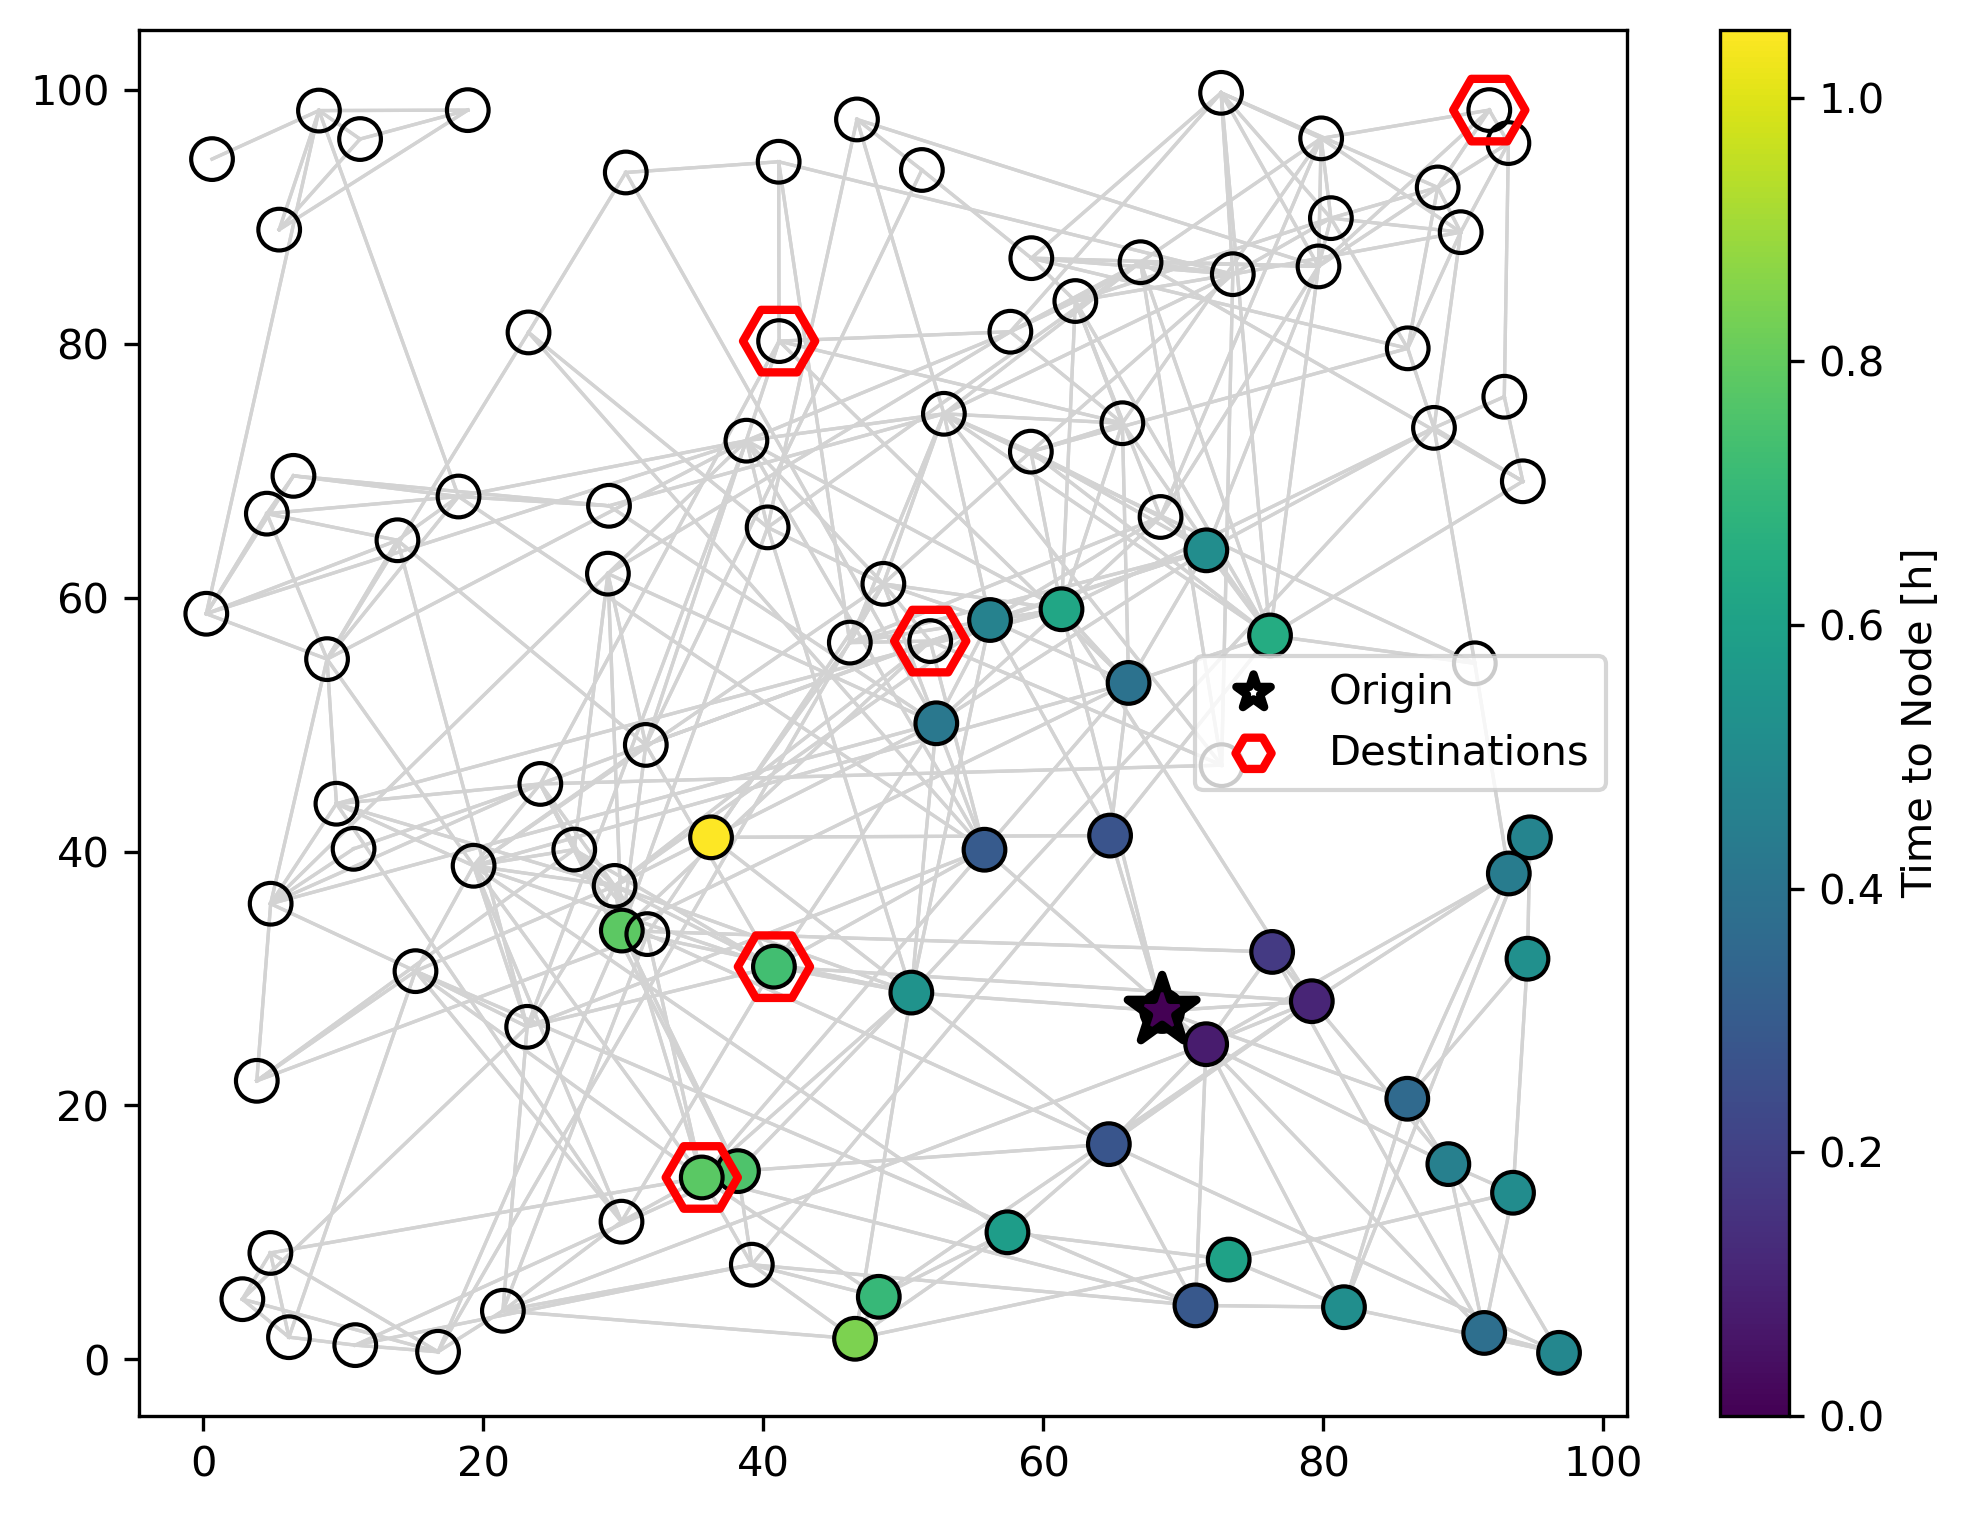
\includegraphics[width = \linewidth]{figs/routing_without_chargers.png}
	\end{subfigure}%
	\begin{subfigure}{.5\linewidth}
		\centering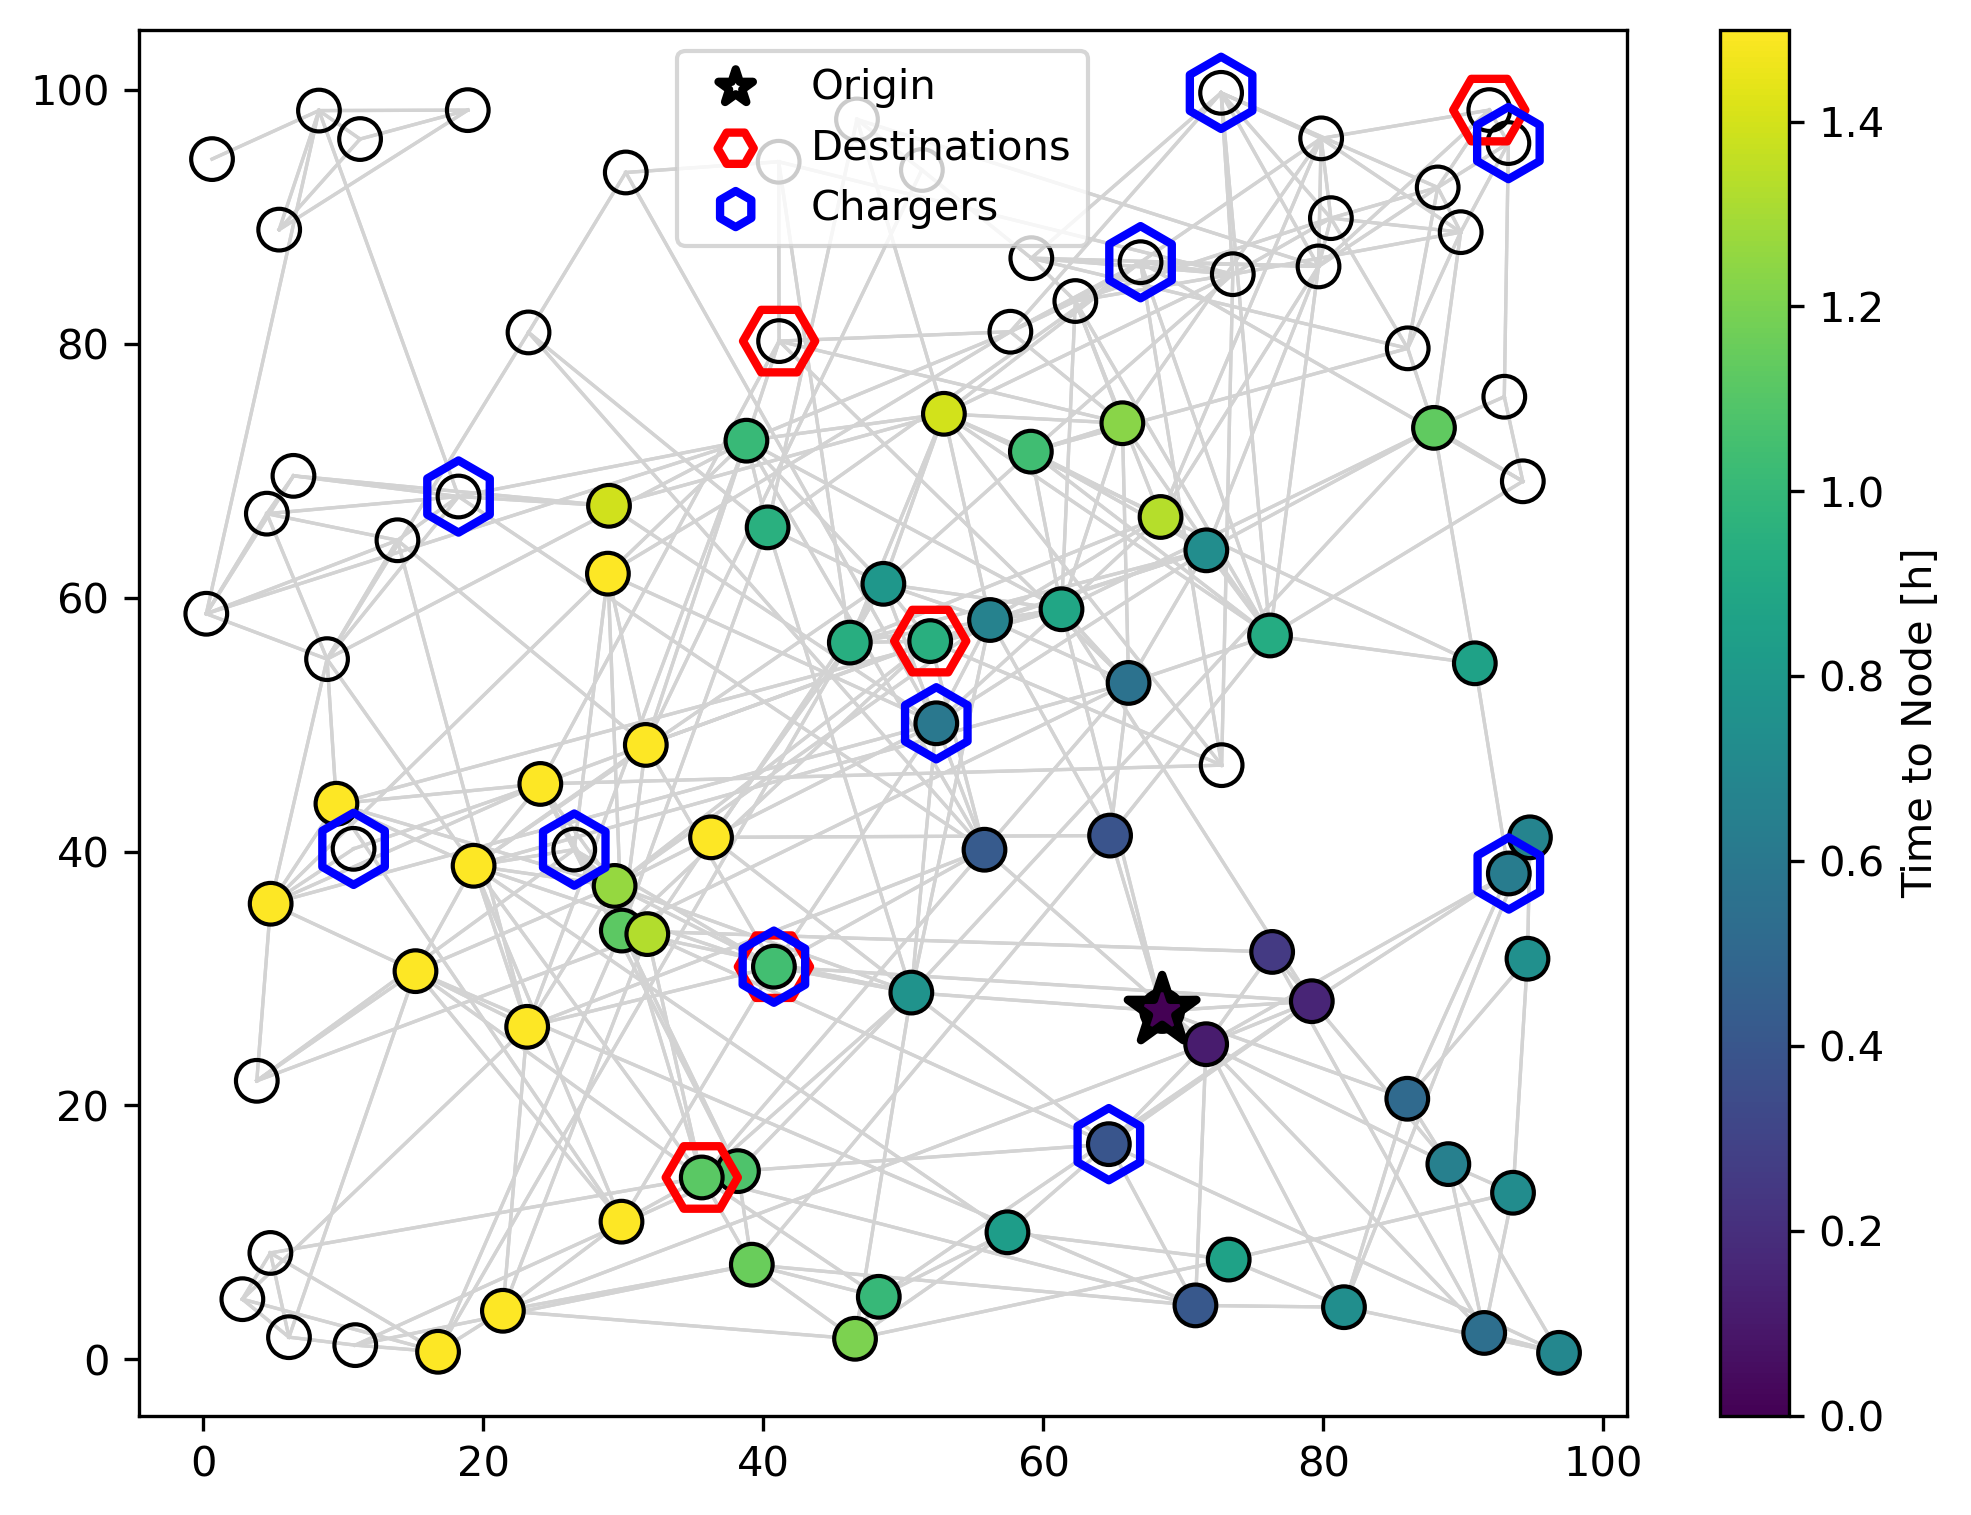
\includegraphics[width = \linewidth]{figs/routing_with_chargers.png}
	\end{subfigure}
	\caption{Routing with (right) and without (left) chargers}
	\label{fig:routing_chargers}
\end{figure}

\subsection*{Stochastic Routing}

The principle of stochastic optimization is to find the set of controls which returns the best expected outcome for an uncertain situation modeled as a set of discrete situations of known likelihood. The goal of stochastic optimization is

\begin{equation}
	\min_{\overline{U}}\quad J(U)=\sum_{S\in\overline{S}} P(S)F(U,S)\label{eq:stochastic_optimization}
\end{equation}

where $\overline{S}$ is the set of possible scenarios, $P(S)$ is the probability of $S$, $F(U,S)$ is the cost of control vector $U$ for scenario $S$, and $\overline{U}$ is the set of possible controls. A control vector $U=\{U_g,U_p\}$ contains general and specific controls (sometimes called first and second stage controls). General controls are shared among all scenarios and specific controls apply only ot one scenario. An example of stochastic optimization is as follows:
\medskip

\framedtext{
\noindent Example - Stochastic Crop Allocation:\\

\noindent A farmer has 100 total acres of fields to plant and may choose from among three crops. Each crop has a different cost per acre for seeds. Depending on meteorological conditions, each crop will have a different revenue per acre in  low, medium, and high yield scenarios. Seeds must be purchased in the fall but the farmer has until the spring to actually decide what to plant and at that point he will have more information about the weather for the coming year. Any excess seeds may be re-sold for a 20\% loss. What quantities of seed should the farmer purchase in order to maximize profit?

\medskip

Discussion:

\medskip

In the example the farmer has to make one set of decisions (what quantities of seeds to buy for the three crops) which holds for all yield scenarios. These are general controls. The farmer then has a set of decisions (what quantities of seed to plant and to resell for each crop) which may vary in different yield scenarios. These are specific controls. The problem contains 3 general controls and 9 specific controls (3 per scenario) for a total of 12 controls. The expected profit for the farmer at the time of seed purchase is the total cost from \eqref{eq:stochastic_optimization} over the number of scenarios.

If the farmer had complete information about the following year's weather at the time of seed purchase he could optimize both seed purchase and seed planting for specific scenarios. In this case the farmer could compute optimal controls for each scenario individually (6 specific controls per scenario). The difference between the expected profit from the stochastic optimization and the mean value of the profits from the deterministic optimizations is called the "cost-of-uncertainty" or the "value-of-information".

A few things are worth mentioning specifically. first, the cost-of-uncertainty should be positive (expected profit less than mean profit). In the example, the farmer may have to buy more seeds than he can possibly plant due to uncertainty and have to sell the excess at a loss. In the deterministic scenarios the optimal solution will never call for purchasing more seeds than needed for planting if the resell value is less than the purchase value. It is intuitive to see that the farmer is paying a price for his decision to purchase seeds before it is possible to predict the weather with sufficient accuracy. Second, stochastic optimization reduces to deterministic optimization with the removal of general controls. In other words, a stochastic optimization problem is an optimization problem with at least one general control and need not have any specific controls.}

\bigskip

For a \gls{bev} driving between an origin and a destination the controls relate to where to charge. If there is less than 100\% certainty of a charger being usable (functional, accessible, and available) at the time of arrival to the charger, the optimization becomes stochastic. The technical non-functionality of a given charger may be known to the driver before the trip but accessibility and availability are not likely to be known prior to arrival. When a driver arrives at a charger and becomes aware that the charger is not usable the driver has the following options: (1) Wait at the charger until it becomes available, (2) re-route from current location to destination. If the charger is found to be non-functional or inaccessible then only option (2) is possible. Less than perfect reliability may result in an optimal route which is, otherwise, higher cost than that for perfect reliability. Less than perfect certainty may result in a route which is, otherwise, higher cost than that produced with perfect information. Sufficiently poor reliability/certainty may render a trip infeasible from the start or after several failed charge events.

\subsubsection*{Dijkstra}

Where deterministic routing occurs on a graph $G$, stochastic routing occurs on the spanning set of possible graphs $\overline{G}$ which has infinite cardinality. In reality, optimization must occur over a finite set. Thus stochastic optimization occurs on $\hat{G}\subset\overline{G}$ of cardinality $N$. Higher values of $N$ better approximate $\overline{G}$ at the cost of increased computational load. Dijkstra's method for stochastic routing results in a single general optimal route $R^*$. $R^*$ is found using a Monte-Carlo style solution wherein $N$ integrations are simultaneously computed along the same paths experiencing different parameters along the way. The goal of the optimization is to produce the route with the lowest expected cost $\mathbb{J}^* = F(R^*,\hat{G})$ where $R^*$ is the expected optimal route.

$R^*$ is subject to charger usability for O/D pairs of a greater distance than the vehicle's remaining range. The net result of charging (or fueling etc.) is that the vehicle's range is reset, time is added to the route, and money is added to the route price. Time additions are due to charge time and a possible delay due to queuing. Price additions are due to charge pricing. As such, the chargers in $\hat{G}$ are parameterized by $\hat{\Psi} = \{\Psi_v,\quad \forall v\in V\}$ where $\Psi_v = \{\psi_v^r,\psi_v^p,\psi_v^d,\psi_v^c\}$ which are the range completion of the charge event (the reset range), the charge power, the wait time before charging, and the charging cost respectively. If the vehicle's remaining range is greater than $\psi_v^r$ no charge event will occur. For stochastic optimization, all parameters are sampled from defined distributions each time the charger is visited.

Depending on the configuration of $G$, certain routes may be feasible or infeasible (because they cause the vehicle range to go below a minimum value) potentially creating a discontinuous cost space where the costs of the feasible routes must be considered alongside those of infeasible routes. A probabilistic risk measure, the Super-Quantile provides an elegant solution. The Super-Quantile function for a given distribution is

\begin{equation}
	S_p(D) = \frac{1}{1-p}\int_{p}^{1}Q_\alpha(D)d\alpha
\end{equation}

where $D$ is a given \gls{pdf}, $p\in[0, 1]$ is a probability threshold, and $Q_\alpha$ is the quantile function of a given \gls{pdf} for probability $\alpha$. In effect, the Super-Quantile is the mean of the \gls{pdf} after $p$. For route $R$ on graphs $\hat{G}$ of cardinality $N$, there will be a revealed distribution $D_r$ of remaining range at all points. The remaining range constraint can thus be written as

\begin{equation}
	S_p(-D_r)\geq -r^{min} \label{eq:remaining_range_constraint}
\end{equation}

where $r^{min}$ is the lowest allowable remaining range and $p$ is set by the user. In effect, \eqref{eq:remaining_range_constraint} guarantees that the expected value of the worst $1-p$ portion of outcomes is within the feasible range. General values of other route costs are computed similarly.


\section*{Routing-Based Metrology}

\subsection*{\gls{icev}/\gls{ev} Cost Differential Tree}

\subsection*{Weighted Charger Centrality}

\subsection*{Charger Availability Value-of-Information}


\appendix
\section*{Routing Algorithms}

\noindent A generic formulation of Dijkstra's algorithm is as follows:

\begin{algorithm}[H]
	\caption{Dijkstra Routing Algorithm}
	\begin{algorithmic}
		\State $G = \{V,E\}$ \Comment{Graph consisting of nodes and links}
		\State $C = \{c_e,\quad\forall e \in E\}$ \Comment{Traversal cost corresponding to each link}
		\State $O\in V$ \Comment{Single origin node}
		\State $D\in V$ \Comment{Set of destination nodes}
		\State
		\State $S = \{\}$ \Comment{Set of seen nodes}
		\State $W = \{\infty,\quad\forall v\in V\}$ \Comment{All node weights initialized to infinity}
		\State $P = \{\{\},\quad\forall d\in D\}$ \Comment{Initializing empty path for each destination}
		\State $v=o_0$ \Comment{Start by processing the origin node}
		\While {$D\not\subset S$} \Comment{Iterating while not all destinations have been seen}
			\ForAll{$e\in E$} \Comment{Iterating through links}
				\If{$e_0=v$} \Comment{If a link originates at the current vertex}
					\If{$W_v+C_e<W_{e_1}$} \Comment{Store current path and path cost if it represents savings}
						\State $P_{e_1}=P_{v}\cup \{e_1\}$
						\State $W_{e_1} = W_v+C_e$
					\EndIf
				\EndIf
			\EndFor
			\State $S=S\cup\{v\}$ \Comment{Add current node to set of seen nodes}
			\State $W_t=\infty$
			\ForAll{$u\in E\not\cap S$} \Comment{Find the nearest unseen node for processing}
				\If{$W_u\leq W_c$}
					\State $v=u$
				\EndIf
			\EndFor
		\EndWhile
	\end{algorithmic}
\end{algorithm}

\noindent A generic formulation of Bellman's algorithm is as follows:

\begin{algorithm}[H]
	\caption{Bellman Routing Algorithm}
	\begin{algorithmic}
		\State $G = \{V,E\}$ \Comment{Graph consisting of nodes and links}
		\State $C = \{c_e,\quad\forall e \in E\}$ \Comment{Traversal cost corresponding to each link}
		\State $O\in V$ \Comment{Set of origin nodes}
		\State $D\in V$ \Comment{Single destination node}
		\State
		\State $S = \{\}$ \Comment{Set of seen nodes}
		\State $W = \{\infty,\quad\forall v\in V\}$ \Comment{All node weights initialized to infinity}
		\State $v=d_0$ \Comment{Start by processing the destination node}
			\While {$D\not\subset S$} \Comment{Iterating while not all origins have been seen}
			\ForAll{$e\in E$} \Comment{Iterating through links}
				\If{$e_1=v$} \Comment{If a link terminates at the current vertex}
					\If{$W_v+C_e<W_{e_0}$} \Comment{Store current path if it represents savings}
						\State $W_{e_0} = W_v+C_e$
					\EndIf
				\EndIf
			\EndFor
			\State $S=S\cup\{v\}$ \Comment{Add current node to set of seen nodes}
			\State $W_t=\infty$
			\ForAll{$u\in E\not\cap S$} \Comment{Find the nearest unseen node for processing}
				\If{$W_u\leq W_c$}
					\State $v=u$
				\EndIf
			\EndFor
		\EndWhile
		\State $P = \{\{\},\quad\forall o\in O\}$ \Comment{Initializing empty path for each origin}
		\ForAll{$o\in O$} \Comment{Iterating on origins}
			\State $v=o$
			\While{$v\neq d_0$} \Comment{Iterating until destination is reached}
				\State $W_t=\infty$
				\State $V_t=\{\}$
				\ForAll{$e\in E$} \Comment{Finding the closest successor node}
					\If{$e_0=v$}
						\If{$W_{e_0}\leq W_t$}
							\State $V_t=\{e_0\}$
						\EndIf
					\EndIf
				\EndFor
				\State $P_v=P_v\cup V_t$ \Comment{Adding closest successor node to path}
			\EndWhile
		\EndFor
	\end{algorithmic}
\end{algorithm}







\end{document}